\documentclass[tikz,border=6pt]{standalone}
\usepackage[T1]{fontenc}
\usepackage{lmodern}
\usetikzlibrary{arrows.meta,positioning,shapes.geometric,fit,calc,backgrounds}
\definecolor{ink}{HTML}{292642}
\definecolor{violet}{HTML}{7054DC}
\definecolor{violetlight}{HTML}{F1EDFF}
\definecolor{teal}{HTML}{147D77}
\definecolor{teallight}{HTML}{E8F5F3}
\definecolor{amber}{HTML}{9A641F}
\definecolor{amberlight}{HTML}{FFF3DE}
\definecolor{linegray}{HTML}{A7A9BA}
\tikzset{box/.style={draw=violet!55,fill=violetlight,rounded corners=3pt,minimum width=2.25cm,minimum height=0.8cm,align=center,font=\sffamily\scriptsize,text=ink,inner sep=5pt},actual/.style={box,draw=teal!70,fill=teallight},proposed/.style={box,dashed,draw=amber!75,fill=amberlight},small/.style={font=\sffamily\tiny,text=ink,align=center},lab/.style={font=\sffamily\scriptsize\bfseries,text=ink},flow/.style={-{Stealth[length=2mm]},line width=.8pt,draw=violet},dflow/.style={flow,dashed,draw=amber},boundary/.style={draw=linegray,dashed,rounded corners=4pt,inner sep=8pt}}
\begin{document}

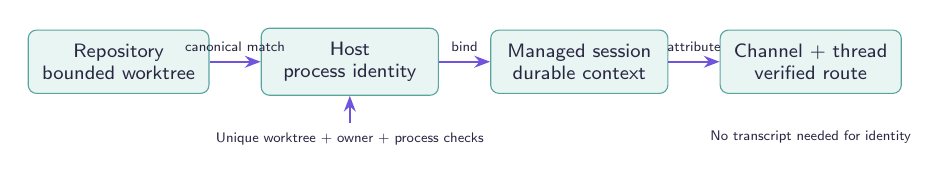
\begin{tikzpicture}[node distance=1.0cm and .65cm]
\node[actual] (repo) {Repository\\bounded worktree};
\node[actual,right=of repo] (host) {Host\\process identity};
\node[actual,right=of host] (session) {Managed session\\durable context};
\node[actual,right=of session] (route) {Channel + thread\\verified route};
\draw[flow] (repo)--node[above,small]{canonical match} (host);
\draw[flow] (host)--node[above,small]{bind} (session);
\draw[flow] (session)--node[above,small]{attribute} (route);
\node[small,below=.35cm of host] (gate) {Unique worktree + owner + process checks};
\node[small,below=.35cm of route] {No transcript needed for identity};
\draw[flow] (gate.north)--(host.south);
\end{tikzpicture}
\end{document}
